\documentclass{scrreprt}
\usepackage{listings}
\usepackage{underscore}
\usepackage[bookmarks=true]{hyperref}
\usepackage[utf8]{inputenc}
\usepackage[english]{babel}
\usepackage{tikz}
\usepackage{xcolor}
\usepackage{graphics}

\usetikzlibrary{shapes.geometric, arrows}
\definecolor{orange}{HTML}{eeeeee}
\hypersetup{
    bookmarks=false,    % show bookmarks bar?
    pdftitle={Design Document},    % title
    pdfauthor={Anjali Venugopal},                     % author
    pdfsubject={TeX and LaTeX},                        % subject of the document
    pdfkeywords={TeX, LaTeX, graphics, images}, % list of keywords
    colorlinks=true,       % false: boxed links; true: colored links
    linkcolor=blue,       % color of internal links
    citecolor=black,       % color of links to bibliography
    filecolor=black,        % color of file links
    urlcolor=purple,        % color of external links
    linktoc=page            % only page is linked
}%

\date{}
%\title
\usepackage{hyperref}

\tikzstyle{process} = [rectangle, minimum width=4.4cm, minimum height=1cm, text centered, draw=black, fill=orange]
\tikzstyle{arrow} = [thick,->,>=stealth]

\begin{document}

\begin{flushright}
    \rule{16cm}{5pt}\vskip1cm
    \begin{bfseries}
        \Huge{DESIGN DOCUMENTATION}\\
        \vspace{1.9cm}
        for\\
        \vspace{1.9cm}
        Hand Gesture GUI Control System\\
        \vspace{1.9cm}
        \LARGE
        Prepared by \\MDL15CS040 19 George Thomas Shanti
        \\MDL15CS082 46 Prince Mathew
        \\MDL15CS089 51 Riza Salahuddin\\
        \vspace{1.9cm}
        \today\\
    \end{bfseries}
\end{flushright}

\tableofcontents


\chapter{Introduction}
section{Purpose}
Hand Gesture GUI Control System version 1 revison 1 - A Real time dynamic Hand Gesture Recognition GUI system to improve the interaction between user and computer. The user can use his webcam to record hand gestures which our system can use to perform Linux GUI functions in realtime.

\section{Overview}
  The Sytem Architecture provides a view into how the different blocks of the system is organized.
  There are mainly four stages in this system. They are Background Subtraction, Feature Extraction,
  Finger-Tip Tracking, Gesture Recognition and Gesture Mapping.\\
  The Video input feed is split into frames and the hand gesture is detected from the multiple frames.
  \\ The User case diagram has the different functions which are targeted at different user classes.
  \\The class structure has been described in the class diagram. There is a main abstract class from which two 
  sub-classes are derived; SavedGestures and DetectedGestures. \\
  The flow of activity has been shown in the activity diagram. All the actions from the start, i.e the user gesture to the mapping and execution of the LINUX GUI function has been shown.
  \\The algorithms section describe the different algorithms used in the system.
  Convex Hull, Camshift and GMG are the main algorithms used.
  


\chapter{System Architecture}
In this section, explain the detailed architecture of the proposed system.
It should include the architecture diagram and the explanation of the modules of the system.
\\
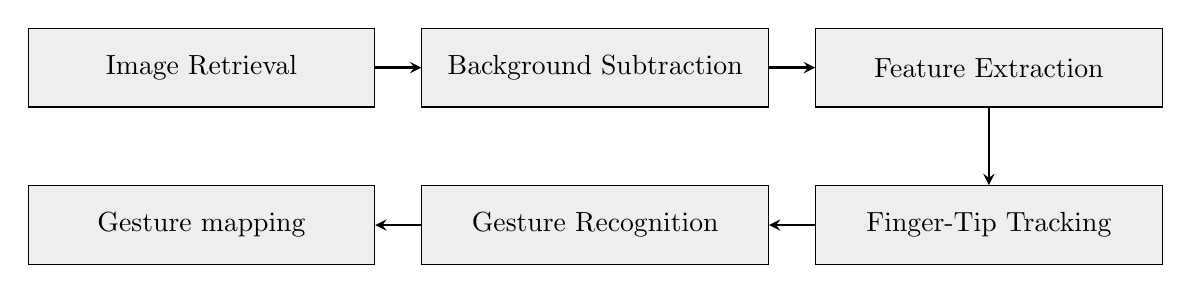
\begin{tikzpicture}[node distance=5cm]
    \node (proc1) [process] {Image Retrieval};
    \node (proc2) [process, right of = proc1] {Background Subtraction};
    \node (proc3) [process, right of = proc2] {Feature Extraction};
    \node (proc4) [process, below of = proc3, yshift = 3cm] {Finger-Tip Tracking};
    \node (proc5) [process, left of = proc4] {Gesture Recognition};
    \node (proc6) [process, left of = proc5] {Gesture mapping};
    \draw [arrow] (proc1) -- (proc2);
    \draw [arrow] (proc2) -- (proc3);
    \draw [arrow] (proc3) -- (proc4);
    \draw [arrow] (proc4) -- (proc5);
    \draw [arrow] (proc5) -- (proc6);
\end{tikzpicture}

\section{Module 1 - Image Retrieval}
The camera feed is retrieved from the user's webcam using the CaptureFromCAM function provided by OpenCV.

\section{Module 2 - Background Subtraction}
The Mixture of Gaussians (MOG) method is used for foreground detection, and once the foreground is detected, we subtract the rest of the image, i. e., the background.

\section{Module 3 - Feature Extraction}
The locations of the fingertips on the screen are detected by finding the Convex hull of the hand and marking the peaks. This process is done in realtime and the extracted location changes with every frame.

\section{Module 4 - Finger-Tip Tracking}
Continuously Adaptive Mean Shift Algorithm (CAMShift) is used to detect the changes from frame to frame. The probability distribution of the first frame is taken as a reference for the second frame, the probability distribution of the second frame is taken for the third frame and so on and so forth.

\section{Module 5 - Gesture Recognition}
The convex hull and convexity defects along with the results of the CAMShift algorithm are used to create a mathematical state of the currently recorded gesture. This state is compared with the states of the saved gestures and the closest candidiate is chosen.

\section{Module 6 - Gesture Mapping}
Once the correct gesture has been identified, the corresponding class object is accessed to procure the GUI function that has been saved for that particular gesture. The function is first executed, and then the daemon starts listening for the next gesture.

\chapter{Data Description}

\section{Data Flow Diagram}

\subsection{Level 0}
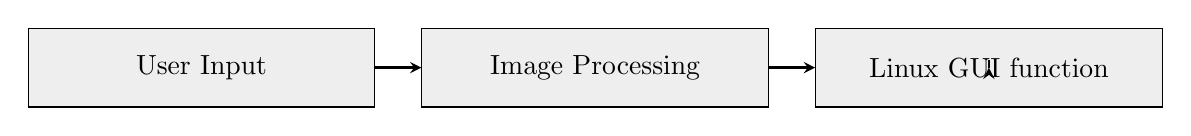
\begin{tikzpicture}[node distance=5cm]
    \node (proc1) [process]{User Input};
    \node (proc2) [process, right of = proc1]{Image Processing};
    \node (proc3) [process, right of = proc2]{Gesture Recognition};
    \node (proc4) [process, right of = proc2]{Linux GUI function};
    \draw[arrow] (proc1)--(proc2);
    \draw[arrow] (proc2)--(proc3);
    \draw[arrow] (proc3)--(proc4);
\end{tikzpicture}

\section{Use case diagram}
\begin{center}
    \includegraphics{usecase.png}
\end{center}
\section{Class diagram}
\begin{center}
    \includegraphics[scale=0.8]{classdiagram.png}
\end{center}
\section{Activity diagram}
\begin{center}
    \includegraphics[scale=0.8]{activitydiagram.png}
\end{center}

\chapter{Algorithms}
Explain the pseudocodes of the algorithms that will be used in the implementation of the project.
\section{Algorithm 1}
psuedocode and its explanation briefly.
\section{Algorithm 2}
psuedocode and its explanation briefly.
\begin{thebibliography}{999}
\addcontentsline{toc}{chapter}{References}

\bibitem{} 
\bibitem{}

\bibitem{} 

\bibitem{} 

\bibitem{} 

\bibitem{} 



\end{thebibliography}

\end{document}